\documentclass[10pt,twocolumn]{article}

% ---------- Packages ----------
\usepackage[utf8]{inputenc}
\usepackage[T1]{fontenc}
\usepackage[a4paper,margin=0.75in]{geometry}
\usepackage{graphicx}
\usepackage{amsmath,amssymb}
\usepackage{booktabs,tabularx,array}
\usepackage{enumitem}
\usepackage{microtype}
\usepackage{xcolor}
\usepackage[most]{tcolorbox}
\usepackage{listings}
\usepackage{tikz}
\usetikzlibrary{arrows.meta,positioning,shapes.geometric,fit}
\usepackage[numbers,sort&compress]{natbib}
\usepackage{url}
\usepackage{hyperref}
\usepackage{cleveref}
\usepackage{parskip}

\hypersetup{
  colorlinks=true,
  linkcolor=blue!60!black,
  citecolor=green!40!black,
  urlcolor=blue!60!black
}

\setlist[itemize]{leftmargin=*,nosep}
\setlist[enumerate]{leftmargin=*,nosep}
\newcolumntype{Y}{>{\raggedright\arraybackslash}X}

\lstset{
  basicstyle=\ttfamily\scriptsize,
  breaklines=true,
  frame=single,
  columns=fullflexible,
  showstringspaces=false
}


% ---------- Definition boxes ----------
\newtcolorbox{definitionbox}[1]{
  colback=blue!2,
  colframe=blue!35!black,
  boxrule=0.55pt,
  arc=1.2mm,
  left=1.5mm,right=1.5mm,top=1.2mm,bottom=1.2mm,
  title=\textbf{#1},
  fonttitle=\normalsize,
  before skip=4pt,after skip=4pt
}

\newtcolorbox{subdefinitionbox}[1]{
  colback=white,
  colframe=black!35,
  boxrule=0.4pt,
  arc=1mm,
  left=1.2mm,right=1.2mm,top=1mm,bottom=1mm,
  title=\textbf{#1},
  fonttitle=\small,
  before skip=3pt,after skip=2pt
}

% ---------- Title ----------
\title{\textbf{Context-Aware Retrieval-Augmented Synthesis of Land--Atmosphere Literature for Land-Use Scenario Design, with a Proposed Regional Climate Modelling Use Case}}
\author{ICTD, IIT Delhi}
\date{}

\begin{document}
\maketitle

\begin{abstract}
Land-use and land-cover change (LULCC) modifies the exchange of energy, moisture and momentum between the land surface and atmosphere, and can therefore alter near-surface temperature, boundary-layer development, cloud formation, precipitation and circulation from local to remote scales. The sign and magnitude of these effects are strongly context dependent: the response to afforestation, deforestation, irrigation, cropland expansion, wetland or lake restoration, paddy cultivation, or other land interventions depends on background hydroclimate, atmospheric state, soil moisture, vegetation characteristics, spatial heterogeneity, patch scale, terrain and advection. This context dependence makes direct translation from individual studies to local planning difficult.

Running many alternative LULC experiments with numerical weather or climate models is computationally expensive. We therefore developed a literature-retrieval framework that identifies evidence-grounded LULC interventions, mechanisms, outcomes and spatial conditions, allowing a smaller set of plausible scenarios to be selected for further study. We consider three literature-retrieval systems: (i) a conventional passage-based RAG baseline, (ii) Microsoft GraphRAG, and (iii) a custom context-aware land--atmosphere knowledge-graph RAG. The custom system represents study Contexts, ContextVariables, interventions, evidence-backed Claims, canonical States and exact source provenance. NVIDIA Nemotron Parse v1.2 is used for PDF parsing, Qwen3.6:27b through Ollama for semantic extraction, and Qwen3 embeddings for retrieval. During querying, the environmental conditions of the target area are compared with those reported in the literature before Claims are combined into mechanism chains.

The present work focuses on the retrieval and reasoning system. A suggested downstream application is to convert selected RAG-generated LULC suggestions into spatially explicit raster scenarios and evaluate those scenarios with a numerical weather prediction model such as WRF. This would allow literature-derived hypotheses to be examined under the meteorological and land-surface conditions of a target region. The Results and Discussion sections are reserved for comparison of the three RAG approaches and the effects of retrieval, embedding and language-model parameters.
\end{abstract}

\section{Introduction}

Land surface conditions actively influence the climate system. Changes in vegetation, soil moisture, surface roughness, albedo, rooting depth and evapotranspiration alter the surface energy and water budgets and can influence boundary-layer thermodynamics, convection, precipitation and circulation \cite{pielke2007,cao2020,spracklen2018}. Classical sensitivity experiments illustrate this coupling: large-scale Amazon deforestation has been simulated to warm the surface while reducing evapotranspiration, precipitation and moisture-flux convergence \cite{shukla1990}; Sahelian desertification experiments produced rainfall and circulation changes, including a southward displacement of the rainfall maximum \cite{xue1993}; and irrigation expansion has been associated with substantial cooling of hot extremes in strongly irrigated regions, particularly South Asia \cite{thiery2020}. Together, these examples show that LULCC can influence climate and that the response depends on the land transition and environmental setting.

The scientific difficulty is that land--atmosphere effects are conditional. Forest expansion may increase low-level cloudiness in many environments but the response varies geographically, seasonally and by forest type \cite{duveiller2021}. Soil-moisture heterogeneity can organize convection at scales of tens of kilometres \cite{taylor2011}, while the sign and preferred location of precipitation can change with background wind and convective propagation \cite{froidevaux2014}. Vegetation feedbacks can even reverse between daytime and nighttime because the relevant boundary-layer and convective processes differ \cite{klein2017}. At broader scales, evapotranspired moisture may be transported to distant precipitation sinks, motivating the concepts of moisture recycling and precipitationsheds \cite{keys2012,keys2016,wangerlandsson2018}. A useful planning question is therefore \emph{``under which environmental and spatial conditions, through which supported mechanism, and at what scale might afforestation influence rainfall in this particular region?''}


This study develops the retrieval component of such a framework. The central idea is shown in \cref{fig:framework}: scientific literature is indexed into one of three RAG systems and queried for location-conditioned LULC interventions, mechanisms and outcomes. Selected suggestions can later be converted into explicit raster LULC scenarios and examined with a numerical weather prediction model such as WRF. The framework complements an earlier research roadmap focused on the physical pathways and spatial scales through which LULCC affects regional climate.

\begin{figure*}[t]
\centering
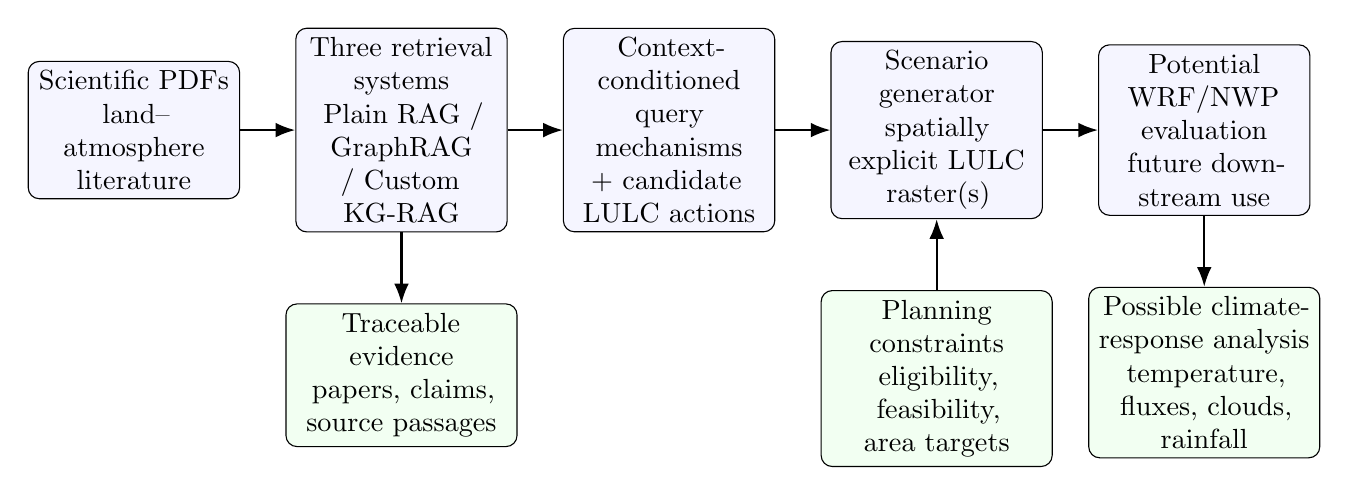
\begin{tikzpicture}[
  node distance=7mm and 7mm,
  box/.style={draw,rounded corners,align=center,minimum height=10mm,text width=2.45cm,fill=blue!4},
  small/.style={draw,rounded corners,align=center,minimum height=9mm,text width=2.7cm,fill=green!5},
  arrow/.style={-{Latex[length=2.5mm]},thick}
]
\node[box] (papers) {Scientific PDFs\\land--atmosphere literature};
\node[box,right=of papers] (rag) {Three retrieval systems\\Plain RAG / GraphRAG / Custom KG-RAG};
\node[box,right=of rag] (query) {Context-conditioned query\\mechanisms + candidate LULC actions};
\node[box,right=of query] (scenario) {Scenario generator\\spatially explicit LULC raster(s)};
\node[box,right=of scenario] (wrf) {Potential WRF/NWP evaluation\\future downstream use};
\draw[arrow] (papers)--(rag);
\draw[arrow] (rag)--(query);
\draw[arrow] (query)--(scenario);
\draw[arrow] (scenario)--(wrf);
\node[small,below=9mm of rag] (evidence) {Traceable evidence\\papers, claims, source passages};
\node[small,below=9mm of scenario] (constraints) {Planning constraints\\eligibility, feasibility, area targets};
\node[small,below=9mm of wrf] (outcomes) {Possible climate-response analysis\\temperature, fluxes, clouds, rainfall};
\draw[arrow] (rag)--(evidence);
\draw[arrow] (constraints)--(scenario);
\draw[arrow] (wrf)--(outcomes);
\end{tikzpicture}
\caption{Conceptual workflow. The present work focuses on retrieving evidence-grounded candidate interventions and mechanisms. Raster scenario construction and WRF/NWP experiments illustrate a possible downstream application of these outputs.}
\label{fig:framework}
\end{figure*}


\section{Definitions}
\label{sec:definitions}

The custom retrieval system uses a small set of scientific objects. The definitions below follow their hierarchy. Fields that belong to an object are shown inside the corresponding box.

\paragraph{Paper.}
A \texttt{Paper} is one scientific publication included in the indexed literature corpus. It provides study-level provenance for the Contexts, ContextVariables, Transitions and Claims extracted from that publication.

\begin{definitionbox}{SourceBlock}
A \texttt{SourceBlock} is a stable passage of text from a parsed paper. It is the smallest source unit retained for provenance, so an extracted object or final answer can be traced back to the exact supporting passage.

\textbf{Example.} A paragraph reporting that forest replacement reduced evapotranspiration and precipitation can be stored as \texttt{SB\_0142}. A Claim extracted from that paragraph keeps \texttt{SB\_0142} as its direct evidence.
\end{definitionbox}

\begin{definitionbox}{Context}
A \texttt{Context} represents the complete environmental, experimental or scenario setting under which a study result is interpreted. It can correspond to a study region and season, a control or perturbation experiment, a daytime or nighttime regime, or a particular atmospheric-flow condition. Each extracted result is associated with the Context in which it was reported.

\textbf{Example.} A Context may represent a \emph{Sahel wet-season convective environment with heterogeneous soil moisture and weak synoptic forcing}.

\begin{subdefinitionbox}{Parent and child Contexts}
A \texttt{parent Context} contains background conditions shared by several more specific cases. A \texttt{child Context} inherits those shared ContextVariables and adds the conditions that differ or become more specific.

\textbf{Example.}
\begin{itemize}
  \item \textbf{Parent:} \texttt{CTX\_SAHEL\_WET} --- Sahel wet season, semi-arid surface, heterogeneous soil moisture.
  \item \textbf{Child A:} \texttt{CTX\_DAY} --- inherits the parent conditions and adds \emph{daytime convective regime}.
  \item \textbf{Child B:} \texttt{CTX\_NIGHT} --- inherits the same parent conditions and adds \emph{nighttime convective regime}.
\end{itemize}
The day and night Claims can therefore remain separate while retaining their common environmental background.
\end{subdefinitionbox}
\end{definitionbox}

\begin{definitionbox}{ContextVariable}
A \texttt{ContextVariable} describes one coherent characteristic of a Context. Examples include background wind regime, soil-moisture heterogeneity, land-cover composition, terrain setting, or patch configuration. A ContextVariable can contain qualitative and quantitative information together in one scientific description.

\textbf{Example.} A ContextVariable can describe the \emph{background wind regime} of a convective experiment, including the flow strength, atmospheric level and its role in transporting convection from one land-surface patch to another.
\end{definitionbox}

\begin{subdefinitionbox}{ContextVariable fields}
The following fields are contained within each \texttt{ContextVariable}:

\textbf{domain} --- broad scientific family used to group comparable variables. \textbf{Example:} \texttt{atmosphere}.

\textbf{name} --- short open-vocabulary label for the variable. \textbf{Example:} \texttt{background wind regime}.

\textbf{description} --- evidence-grounded scientific detail, including values, ranges, units, seasonality, direction or spatial relations when relevant. \textbf{Example:} \emph{Moderate mid-tropospheric flow permits convection initiated over dry patches to propagate into wetter patches.}

\textbf{origin} --- how the variable entered the system, such as directly reported in the paper or derived from an environmental dataset. \textbf{Example:} \texttt{reported}.

\textbf{evidence} --- provenance supporting the variable. For reported variables this is one or more SourceBlock identifiers; for derived variables it records the dataset and derivation metadata. \textbf{Example:} \texttt{SB\_031--SB\_033}.
\end{subdefinitionbox}

\begin{definitionbox}{Transition}
A \texttt{Transition} represents a comparison or intervention connecting two Contexts. It is used when a study explicitly changes the land surface, management state, or experimental condition and evaluates the resulting response.

\textbf{Example.} \texttt{forest Context $\rightarrow$ degraded-pasture Context} represents the deforestation experiment, while \texttt{non-irrigated Context $\rightarrow$ irrigated Context} represents an irrigation intervention.
\end{definitionbox}

\begin{definitionbox}{State}
A \texttt{State} is a compact, reusable scientific endpoint used to connect findings across papers. It contains a scientific concept and the reported direction or categorical state of that concept.

\textbf{Example.} \texttt{evapotranspiration :: decrease}, \texttt{precipitation :: increase}, or \texttt{near-surface air temperature :: increase}.
\end{definitionbox}

\begin{definitionbox}{Claim}
A \texttt{Claim} is one evidence-supported relationship between two States. It remains attached to the Context or Transition in which the relationship was reported and retains the SourceBlocks that support it. The associated Context records the conditions under which the relationship was observed, simulated or inferred in the paper.

\textbf{Example.}
\begin{quote}\small
\texttt{from}: evapotranspiration :: decrease\\
\texttt{to}: precipitation :: decrease\\
\texttt{relation}: causal\\
\texttt{applies to}: Amazon forest-to-pasture Transition
\end{quote}

\begin{subdefinitionbox}{Conditioning ContextVariables}
Some Claims depend especially strongly on particular variables within their Context. The field \texttt{conditioning\_context\_variable\_ids} records those variables so that they receive additional attention when a Claim is compared with a new query area.

\textbf{Example.} For a soil-moisture--precipitation Claim whose sign changes between weak- and strong-flow experiments, the \emph{background wind regime} ContextVariable can be recorded as a conditioning variable.
\end{subdefinitionbox}
\end{definitionbox}

\begin{definitionbox}{Query Context}
A \texttt{Query Context} is the temporary Context created for the user's target area or question. It uses the same ContextVariable representation as the indexed studies, allowing the environmental conditions of the target area to be compared directly with those reported in the literature.

\textbf{Example.} For a query about afforestation in a semi-arid watershed, the Query Context may contain ContextVariables describing the seasonal climate, current land cover, soil-moisture regime, terrain, prevailing wet-season flow and proposed intervention geometry, where those variables are supplied by the user or derived from configured datasets.
\end{definitionbox}

\section{Scientific Basis: Mechanisms and Spatial Scales}

\subsection{Surface-energy and moisture pathways}

LULCC modifies climate through coupled radiative, turbulent, hydrological and dynamical pathways. Vegetation and land management alter albedo, canopy resistance, aerodynamic roughness, rooting depth, soil-water access and evapotranspiration. These properties control the partitioning of net radiation into latent and sensible heat fluxes and therefore modify near-surface temperature and the evolution of the atmospheric boundary layer \cite{spracklen2018}. In the Amazon deforestation experiment of Shukla et al. \cite{shukla1990}, replacing forest with degraded pasture simultaneously changed albedo, surface roughness, stomatal resistance, rooting characteristics and soil-water storage. The representation therefore records the land transition together with the environmental and surface properties relevant to the reported response.

Irrigation and paddy cultivation provide complementary examples. Irrigation can increase surface water availability and latent heat flux and can substantially suppress hot extremes in strongly irrigated regions \cite{thiery2020}. Recent satellite-based mapping of paddy rice indicates growing-season daytime land-surface cooling relative to other croplands, with stronger cooling in larger paddy fields and partial spillover to surrounding landscapes \cite{weng2025}. Conversely, large photovoltaic installations can alter albedo, vegetation, surface energy storage and turbulent flux partitioning; empirical observations have reported a nighttime photovoltaic heat-island effect relative to nearby wildlands \cite{barrongafford2016}. These different interventions motivate a retrieval representation that can describe both the land transition and the physical response without assuming that all LULCC follows one mechanism.

\subsection{Heterogeneity, patch scale, edge effects and advection}

Landscape patterning is important because heterogeneous surface fluxes can organize mesoscale circulations. Observational and modelling work has linked landscape heterogeneity to thermally induced circulations and convective organization \cite{weaver2001}. Large-eddy simulations show that the strength of organized motions depends on the ratio of the heterogeneity scale to boundary-layer depth; Patton et al. \cite{patton2005} found strongest patch-induced motions for intermediate normalized scales. Taylor et al. \cite{taylor2011} found that Sahelian storm initiation was strongly associated with soil-moisture gradients at approximately 10--40 km scales. Such evidence suggests that the climatic influence of an intervention can depend on fractional area, patch size, contrast, edge density and location relative to the prevailing flow.

Directional effects are likewise mechanism dependent. Froidevaux et al. \cite{froidevaux2014} showed that sufficiently strong flow can allow convection initiated over dry patches to propagate toward wetter patches and intensify, whereas weak flow can produce a different feedback sign and rainfall location. Rabin et al. \cite{rabin1990} documented preferred cloud development and suppression relative to heterogeneous land surfaces and downwind bands under weak synoptic forcing. At larger distances, Cohn et al. \cite{cohn2019} found non-local warming associated with forest loss at distances out to 50 km in Brazil. We therefore distinguish local advection, patch-edge circulation, distance decay, terrain-flow interaction and remote moisture recycling as separate spatial relation types.

\subsection{Remote moisture recycling and teleconnections}

Land influence can extend beyond the local boundary layer. Terrestrial evaporation contributes moisture to downwind precipitation, and precipitationsheds describe the upwind land and atmosphere contributing evaporation to a precipitation sink \cite{keys2012}. Vegetation-regulated moisture recycling has been framed as an ecosystem service with geographically separated source and beneficiary regions \cite{keys2016}. Wang-Erlandsson et al. \cite{wangerlandsson2018} further showed that remote land-use change can affect river flows through atmospheric moisture pathways. Precipitationshed boundaries are probabilistic and time dependent. Remote moisture-source questions are therefore represented using source--sink moisture relationships, while local upwind/downwind questions use local flow information.

These spatial and mechanistic complexities motivate the context-aware retrieval design described below.

\section{Research Questions and System Objectives}

The proposed system is intended to answer questions posed by local planners, adaptation scientists, engineers and researchers, including:

\begin{itemize}
  \item What climatic effects are reported when a particular land-cover transition is implemented?
  \item What land-use interventions could plausibly reduce hot extremes, increase cloudiness, alter rainfall, or modify other target outcomes in a given area?
  \item Could intervention $A$ influence outcome $B$, and through which evidence-supported mechanism chain?
  \item Where should an intervention be located relative to prevailing winds, terrain, existing land cover or a target watershed?
  \item At what spatial scale or distance has an effect been observed or simulated?
  \item Which findings from other regions are environmentally analogous enough to be considered transferable to the target context?
  \item Where does the literature disagree, reverse sign, or remain under-constrained?
\end{itemize}

The retrieval system organizes paper-supported evidence, compares study conditions with a target area, reconstructs supported mechanism chains, and proposes candidate LULC scenarios for further investigation. Physical climate response can subsequently be examined with numerical modelling when appropriate.

\section{Retrieval Systems Evaluated}

We compare three RAG configurations using the same literature corpus and query set.

\begin{table*}[t]
\centering
\caption{Retrieval systems included in the planned comparison.}
\label{tab:ragcompare}
\begin{tabularx}{\textwidth}{p{2.6cm}YYY}
\toprule
\textbf{System} & \textbf{Index representation} & \textbf{Query behaviour} \\
\midrule
Plain RAG & Source passages/chunks with dense and/or lexical retrieval & Retrieve top-$k$ passages and synthesize an answer from retrieved evidence \cr
Microsoft GraphRAG & Generic entity--relationship graph, communities and graph-derived summaries \cite{edge2024} & Graph-supported local/global retrieval and query-focused summarization  \cr
Custom context-aware KG-RAG & Paper, Context, ContextVariable, Transition, Claim, State and SourceBlock graph & Compare the Query Context with paper Contexts, select relevant Claims, and search supported mechanism paths  \cr
\bottomrule
\end{tabularx}
\end{table*}

Conventional RAG combines generation with an external retrieval memory \cite{lewis2020} and provides a passage-level baseline. Microsoft GraphRAG builds a graph over the corpus and supports graph-based summarization \cite{edge2024}. Our custom system adds explicit study Contexts, ContextVariables, Claims and spatial conditions because land--atmosphere relationships can change in sign or magnitude across hydroclimates, seasons, atmospheric regimes and spatial configurations.

\section{Custom Context-Aware Knowledge-Graph RAG}

\subsection{Scientific information represented in the custom system}

The custom system represents each study through a small set of linked scientific objects. Findings are associated with the Context or experimental Transition in which they were reported. Environmental conditions are described by a small number of ContextVariables. Claims connect reusable scientific States and retain direct evidence from the paper. Environmental information reported by a paper and information derived from spatial datasets are recorded with separate provenance.

The main objects are:

\begin{center}
\small
\texttt{Paper -- Context -- ContextVariable -- Transition -- Claim -- State -- SourceBlock}
\end{center}

A \texttt{Context} represents an environmental, experimental or scenario state. Child Contexts inherit the shared ContextVariables of their parent. A \texttt{ContextVariable} contains a broad \texttt{domain}, a short \texttt{name}, a scientific \texttt{description}, its origin and its evidence. A \texttt{Transition} represents a comparison or intervention from one Context to another. A \texttt{Claim} represents one evidence-supported relation between two scientific States and is associated with a Context or Transition. A \texttt{SourceBlock} provides the exact source passage supporting an extracted object.

\subsection{Indexing the literature}
\label{sec:indexing}

The indexing sequence is summarized as:

\begin{center}
\small
\texttt{PDF $\rightarrow$ parse and clean $\rightarrow$ SourceBlocks $\rightarrow$ identify study settings $\rightarrow$ extract Contexts, ContextVariables, Transitions and Claims $\rightarrow$ combine results $\rightarrow$ add spatial-data variables $\rightarrow$ standardize States $\rightarrow$ embeddings and linked index}
\end{center}

\subsubsection{Document parsing and stable evidence blocks}

PDFs are parsed using NVIDIA Nemotron Parse v1.2, selected because the model provides structured document extraction with spatial grounding for text and table elements \cite{nemotronparse}. Parsing is followed by deterministic Markdown cleaning: repeated headers/footers, page artefacts and parse noise are removed while preserving section boundaries, tables, captions and scientific notation. The cleaned document is then segmented into stable SourceBlocks using semantic section boundaries and token limits. SourceBlock identifiers are permanent evidence anchors and are created for every paper, independent of paper length.

SourceBlocks function as evidence units. They are used to assemble compact passages for semantic extraction and later provide the source text for citation and provenance.

\subsubsection{Identifying study settings and comparisons}

A first semantic pass identifies the study areas, major experiments or comparisons, candidate Contexts, candidate Transitions and the parts of the paper that support them. Papers below the configured whole-paper token threshold are read in a single call. Longer papers are first read section by section and the extracted information is then combined. The project uses local \texttt{qwen3.6:27b} inference through Ollama with structured outputs and no/low/medium reasoning settings.

Each study setting is described with a small number of coherent ContextVariables. For example, a ``semi-arid wet-season environment with persistent southwesterly low-level flow'' can be represented by variables describing the hydroclimate, season and background flow. A new Context is used when the paper distinguishes a different state that changes how the results are interpreted, such as forest and pasture experiments, daytime and nighttime responses, or strong-wind and weak-wind cases.

\subsubsection{Extracting ContextVariables}

Allowed ContextVariable domains are:

\begin{center}
\small
\texttt{spatial\_configuration, land\_surface, hydrology, atmosphere, climate, substrate\_terrain, other.}
\end{center}

Each ContextVariable describes one coherent property of the study Context. The \texttt{name} is a short open-vocabulary label (typically a few words), while \texttt{description} preserves the scientifically relevant qualifiers, usually in roughly 20--60 words when needed. The description may contain reported ranges, units, seasonality, spatial relations and directional information. The 20--60 word range is a writing guideline and longer descriptions are retained when scientific qualifiers require them. The Context itself provides the scope of the variable. A separate Context is used when a qualifier defines a distinct experimental or environmental state.

ContextVariables are taken from the paper or from explicitly configured environmental datasets. Geographic names are retained as location information. For example, a study located in Rajasthan receives a semi-arid or monsoonal ContextVariable when that information is reported in the paper or derived from the configured spatial data.

\subsubsection{Extracting Transitions and Claims}

For each experimental comparison or scenario change, the system extracts a Transition and evidence-backed Claims. A Claim has a compact directional or categorical State at each endpoint, a causal/associative relation, a short description preserving important qualifiers, a Context or Transition scope, and exact supporting SourceBlock identifiers. Claims may additionally reference \texttt{conditioning\_context\_variable\_ids}: the subset of ContextVariables within that Context that are materially relevant to interpreting or transferring the Claim.

Each Claim represents a relationship that is directly supported by the paper. If a paper reports only ``forest loss $\rightarrow$ precipitation decrease'', that relationship is stored as one Claim. Separate Claims are added when the paper also provides evidence for changes in evapotranspiration, sensible heat, moisture convergence or boundary-layer state. These supported Claims can later be connected into a longer mechanism chain.

We applied the representation to a heterogeneous pilot corpus spanning deforestation, afforestation, irrigation, paddy cultivation, landscape heterogeneity, soil-moisture feedbacks, distance-decay effects and remote moisture recycling. The corpus includes examples with sign reversals, scale dependence, spatial directionality and multi-step mechanisms, and was used to check whether these features can be retained in the extracted representation. Quantitative retrieval results are reserved for the Results section.

\subsubsection{Selecting source text for extraction}

For each extraction call, the relevant SourceBlocks are selected from the paper map, exact Context terms, BM25 retrieval, semantic retrieval and neighbouring blocks. Results and analysis sections receive higher priority when Claims are extracted, while study-area and methods sections receive higher priority for ContextVariables. Adjacent blocks are kept together when they form one continuous piece of evidence.

Each selected passage is also identified as either a result of the current paper or background information cited from another study. Claims attributed to the current paper are created from passages that report or analyse the current study's own findings.

\subsubsection{Adding environmental information from spatial datasets}

For Contexts with known geometry, additional environmental information can be calculated from configured geospatial products. These variables can include climate class, aridity or hydroclimate, seasonal wind, terrain and LULC composition. Raster values are aggregated using area-weighted statistics. Each derived ContextVariable records the dataset and version, temporal window, geometry hash and algorithm version. Paper-reported variables keep their own provenance.

The same spatial-data calculations are applied to the user's query area. This gives the paper Contexts and Query Context comparable descriptions of climate, terrain, land cover and circulation where those datasets are available.

\subsubsection{Standardizing scientific State names}

ContextVariable domains use a small controlled vocabulary, while their names and descriptions remain open vocabulary. State concepts are standardized more strictly because Claims from different papers connect through shared States. Text normalization and a curated alias registry resolve known equivalents such as ``ET'' and ``evapotranspiration''. Embedding similarity is used to find a small set of possible matches when no exact alias is available. Ambiguous matches remain separate until they can be resolved with sufficient evidence.

\subsubsection{Embeddings and links between extracted objects}

Qwen3 embeddings are generated for ContextVariable names, ContextVariable content, Claims, Context summaries and State concepts. For a ContextVariable $f$, two embeddings are retained:

\begin{align}
E_{\mathrm{name}}(f) &= E(\text{domain} \; | \; \text{name}),\\
E_c(f) &= E(\text{domain, name, description}).
\end{align}

The extracted objects are linked according to their scientific relationships. Important relations include \texttt{HAS\_CONTEXT}, \texttt{PARENT\_OF}, \texttt{HAS\_CONTEXT\_VARIABLE}, \texttt{HAS\_TRANSITION}, \texttt{FROM}, \texttt{TO}, \texttt{HAS\_CLAIM}, \texttt{SCOPED\_TO}, \texttt{CONDITIONED\_BY} and \texttt{SUPPORTED\_BY}.

\subsection{Querying the indexed literature}
\label{sec:querying}

The query is processed as follows:

\begin{center}
\small
\texttt{question $\rightarrow$ Query Context $\rightarrow$ add spatial-data variables $\rightarrow$ retrieve similar Contexts $\rightarrow$ compare ContextVariables $\rightarrow$ select Claims $\rightarrow$ search mechanism chains $\rightarrow$ SourceBlocks $\rightarrow$ cited answer}
\end{center}

\subsubsection{Representing the query}

A query contains a temporary Context using the same ContextVariable representation as the indexed papers, plus optional source and target States and a free-text intervention description. Query mode is assigned deterministically:

\begin{itemize}
  \item \textbf{forward}: $A \rightarrow ?$, e.g. ``what happens if irrigation expands?'';
  \item \textbf{backward}: $? \rightarrow B$, e.g. ``what could reduce hot extremes?'';
  \item \textbf{$A\rightarrow B$}: mechanism/path query, e.g. ``could afforestation increase rainfall?'';
  \item \textbf{global}: literature synthesis without a single local environmental gate.
\end{itemize}

The parser reorganizes information explicitly present in the question into the query schema. Environmental properties come from user-provided information or configured datasets. Where geometry is available, the spatial-data functions derive relevant climate, terrain, LULC, hydrological and circulation ContextVariables.

\subsubsection{Comparing the Query Context with paper Contexts}

Whole-Context embeddings are used to retrieve an initial set of candidate Contexts. The detailed comparison then uses individual ContextVariables. For a query ContextVariable $q$ and candidate ContextVariable $c$, pair similarity is

\begin{equation}
 s(q,c)=\alpha\cos(E_{\mathrm{name}}(q),E_{\mathrm{name}}(c))+(1-\alpha)\cos(E_c(q),E_c(c)),
\end{equation}

where $\alpha$ controls the relative importance of name identity versus descriptive environmental similarity. Within a domain $d$, directional MaxSim is

\begin{equation}
S_d(Q,C)=\frac{1}{|Q_d|}\sum_{q\in Q_d}\max_{c\in C_d}s(q,c).
\end{equation}

Domain scores are combined with configurable weights so each scientific domain contributes in a controlled way. The query report records both the similarity scores and the fraction of query information that could be compared. Missing information is therefore visible separately from low-similarity information. An optional unbalanced optimal-transport comparison can also be evaluated for cases with several unmatched ContextVariables.

\subsubsection{Keeping the different relevance scores separate}

Environmental similarity, intervention similarity and outcome relevance are calculated and reported separately. The query report stores:

\begin{itemize}
  \item Context/environment similarity;
  \item source and target State relevance;
  \item Transition/intervention similarity;
  \item spatial-configuration similarity;
  \item Claim/mechanism relevance;
  \item Context coverage and unmatched query ContextVariables.
\end{itemize}

These scores are used to rank evidence for the query. They are reported separately from any scientific assessment of confidence or uncertainty.

\subsubsection{Selecting Claims before searching for mechanism chains}

The system first retrieves paper Contexts that are similar to the Query Context. Claims associated with those Contexts and Transitions form the evidence available for the query. Mechanism chains are then searched within this selected set of Claims. This sequence keeps each mechanism chain tied to the environmental settings that supported its individual relationships.

For a Claim edge $e$ supported by Context $C_e$, the Claim relevance score uses $S(Q,C_e)$ together with any conditioning ContextVariables. For a mechanism path, we use the minimum Claim relevance along the path:

\begin{equation}
A_{\mathrm{path}} = \min_{e \in \mathrm{path}} A_e(Q),
\end{equation}

The path score also includes the similarity between the Contexts supporting adjacent Claims. Maximum path length, beam width, Context threshold, endpoint thresholds and path-length penalties are recorded as tunable parameters.

\subsubsection{Spatial and directional reasoning}

Spatial relations are handled in several families because they describe different physical processes:

\begin{itemize}
  \item local advection and upwind/downwind transport;
  \item patch-edge and heterogeneity-induced circulation;
  \item windward/leeward terrain interaction;
  \item distance-decay footprints;
  \item moisture-recycling and precipitationshed relations;
  \item remote/large-scale teleconnections.
\end{itemize}

For local advection, the query area can be enriched with seasonal wind vectors and the literature relation can be translated onto the actual geography. For windward/leeward mechanisms, terrain and flow are combined. For patch mechanisms, patch size, edge contrast and orientation are compared. Moisture-recycling relations use an atmospheric moisture-tracking product or model when a geographic source--sink relation is required. Local wind vectors are used for local advection relations. When the available spatial information supports a qualitative relation, the answer reports the qualitative relation together with its evidence.

\subsubsection{Grounding and query reports}

Every substantive scientific sentence in the final answer is traceable through:

\begin{center}
\small
\texttt{answer statement $\rightarrow$ mechanism path/Claim $\rightarrow$ Context and conditioning ContextVariables $\rightarrow$ Paper $\rightarrow$ SourceBlock(s)}.
\end{center}

Along with the natural-language answer, the system produces a machine-readable query report containing matched Contexts, overall and domain similarity, matched and unmatched ContextVariables, intervention relevance, Claim relevance, path scores, supporting evidence and missing information. The report supports inspection of individual retrieval decisions, scientific audit and quantitative evaluation.

\section{From RAG Output to Candidate LULC Scenarios}

A possible downstream use of the RAG output is to translate selected suggestions into one or more \emph{candidate scenarios}. A scenario specification could contain: (i) the baseline land class or management state, (ii) the proposed transition, (iii) the target area or fractional change, (iv) any literature-supported spatial relation such as upwind placement, patch size or distance, (v) season or time horizon if relevant, (vi) the mechanism path motivating the scenario, and (vii) constraints or uncertainty flags.

For example, a query asking how to reduce hot extremes might retrieve irrigation-related cooling evidence \cite{thiery2020}, paddy-related surface cooling \cite{weng2025}, or afforestation evidence depending on the target Context. Selection among retrieved interventions can also incorporate water availability, agricultural suitability, biodiversity, livelihoods, protected areas, legal restrictions and other planning constraints.

\subsection{Raster scenario generation}

If a candidate intervention is selected for downstream testing, a raster scenario could be constructed from a high-resolution baseline LULC map. One possible deterministic workflow is:

\begin{enumerate}
  \item define the target polygon or watershed and load the baseline LULC raster;
  \item construct an eligibility mask excluding water bodies, protected or non-allocatable classes, settlements or other locally specified constraints;
  \item compute a literature-supported spatial preference surface (e.g. upwind sector, edge band, patch-size objective, distance band) when the retrieved evidence and local environmental data provide the required spatial information;
  \item combine this with local planning/suitability layers and allocate pixels until the requested area or fractional change is reached;
  \item generate multiple alternative maps when the literature supports competing spatial configurations or when placement uncertainty is large;
  \item save the modified LULC raster, a change mask, class-area summaries and complete scenario metadata.
\end{enumerate}

In such a workflow, the raster can record two sources of information separately. \emph{Evidence-derived preference} comes from the retrieved literature and mechanism. \emph{Planning-derived feasibility} comes from local constraints, suitability information and participatory planning.

\subsection{Physical consistency of land-surface perturbations}

Some scientific interventions involve changes in more than the categorical LULC class. Forest-to-pasture experiments, for example, may imply changes in albedo, aerodynamic roughness, rooting depth, canopy resistance and water storage simultaneously \cite{shukla1990}. Irrigation includes an explicit water-management change in addition to any vegetation-category change \cite{thiery2020}. Paddy systems include management and seasonal inundation in addition to the cropland category \cite{weng2025}. If these scenarios are later used in a numerical land--atmosphere model, the translation would need to account for whether the intervention is represented adequately by land-cover class alone or also requires changes in land-surface parameters or management processes.

\section{Suggested Downstream Use: Numerical Evaluation with WRF}
\label{sec:wrf_future}

WRF is presented here as a possible downstream application of the retrieval system. The RAG system can produce an evidence-grounded description of a candidate intervention, including the land transition, relevant environmental Context, expected mechanism, reported outcome, spatial scale and any directional or configuration constraints. A later scenario-generation step could translate that description into one or more alternative LULC rasters for a selected study area. Those rasters could then be supplied to a numerical weather or regional climate model such as WRF in a set of control and land-perturbation experiments.

Such experiments could be used to ask whether a literature-supported mechanism is expressed under the target region's meteorological and land-surface conditions. For example, a retrieved hypothesis about irrigation-related cooling, patch-scale convective organization, or afforestation-related cloud changes could be translated into a spatial land scenario and compared with an otherwise equivalent control simulation. The resulting numerical experiment could provide an additional physical test of the scenario. The retrieval score and the simulated climate response would be reported as separate quantities because they answer different questions.

The present study evaluates retrieval quality, Context matching, evidence grounding, mechanism reconstruction and sensitivity to retrieval and model parameters. WRF is presented as a possible downstream application of the generated LULC scenarios. Its configuration, preprocessing and diagnostics would be defined in a subsequent modelling study if that application is pursued.

\section{Evaluation Methodology}

\subsection{Literature corpus and query benchmark}

The evaluation corpus spans several intervention types and mechanism families. The current pilot corpus includes examples of deforestation, afforestation, irrigation, paddy cultivation, desertification, lake/wetland effects, cropland conversion, vegetation variability, patch circulation, soil-moisture gradients, distance decay, downwind effects and remote moisture recycling \cite{shukla1990,duveiller2021,thiery2020,xue1993,taylor2011,froidevaux2014,cohn2019,keys2012,keys2016}. The query benchmark covers forward, backward, $A\rightarrow B$, global and spatial-planning forms.

\subsection{RAG-system comparison}

The three retrieval systems will be evaluated on common PDFs and common queries. Some of the areas of evaluation are mentioned, however, these are limited by domain expertise as it may require a lot of manual checking.

\begin{itemize}
  \item citation/source accuracy and unsupported-statement rate;
  \item correct identification of study Context and intervention;
  \item Context-transfer ranking quality;
  \item accuracy of spatial qualifiers such as patch scale, upwind/downwind and distance;
  \item answer completeness, usefulness and expert interpretability;
  \item latency, token usage and computational cost.
\end{itemize}

\subsection{Model and retrieval parameter comparison}

The evaluation will also compare the effect of key implementation parameters. Planned ablations include Context candidate top-$k$, Claim top-$k$, similarity thresholds, ContextVariable name/content weight $\alpha$ can be compared.


\section{Results}

\emph{The Results section will compare the three RAG systems (plain RAG, Microsoft GraphRAG and the custom context-aware KG-RAG), evaluate retrieval and model parameters, and report evidence-grounding, Context-matching and mechanism-retrieval metrics. The possible WRF application is described separately in \cref{sec:wrf_future}.}

Planned subsections are:
\begin{itemize}
  \item RAG retrieval and citation performance;
  \item Context matching and transferability performance;
  \item mechanism-chain and spatial-reasoning evaluation;
  \item sensitivity to retrieval thresholds, top-$k$, path parameters, embeddings and LLM reasoning settings;
\end{itemize}

\section{Discussion}

\emph{The Discussion will interpret differences among the three retrieval systems and examine which features of the representations and retrieval methods account for those differences. It will also consider literature coverage, contradictory evidence, scale mismatch, parameter sensitivity and the distinction between retrieval scores and scientific uncertainty. The WRF use case will be discussed as a possible extension of the workflow.}
\section{Conclusion}

The proposed methodology uses retrieval-augmented literature synthesis to identify what land--atmosphere mechanisms have been reported, under which environmental conditions, and with what spatial constraints. The custom Context--ContextVariable--Claim representation retains the environmental conditions associated with each piece of evidence as Claims are retrieved and connected across papers. Maintaining plain RAG and Microsoft GraphRAG as baselines makes the value of this additional structure empirically testable. A possible future extension is to translate selected evidence-grounded LULC suggestions into raster scenarios and evaluate them with WRF or another regional numerical model. In this document, WRF is presented as a suggested downstream use of the generated raster scenarios.

% ---------- References ----------
\begin{thebibliography}{99}
\setlength{\itemsep}{0pt}

\bibitem{pielke2007}
Pielke Sr., R. A., Avissar, R., Raupach, M., Dolman, A. J., Zeng, X., \& Denning, A. S. (2007). An overview of regional land-use and land-cover impacts on rainfall. \textit{Tellus B}, 59(3), 587--601. \url{https://doi.org/10.1111/j.1600-0889.2007.00251.x}

\bibitem{cao2020}
Cao, Q., Liu, Y., Georgescu, M., \& Wu, J. (2020). Impacts of landscape changes on local and regional climate: A systematic review. \textit{Landscape Ecology}, 35, 1269--1290. \url{https://doi.org/10.1007/s10980-020-01015-7}

\bibitem{spracklen2018}
Spracklen, D. V., Baker, J. C. A., Garcia-Carreras, L., \& Marsham, J. H. (2018). The effects of tropical vegetation on rainfall. \textit{Annual Review of Environment and Resources}, 43, 193--218. \url{https://doi.org/10.1146/annurev-environ-102017-030136}

\bibitem{shukla1990}
Shukla, J., Nobre, C., \& Sellers, P. (1990). Amazon deforestation and climate change. \textit{Science}, 247, 1322--1325. \url{https://doi.org/10.1126/science.247.4948.1322}

\bibitem{xue1993}
Xue, Y., \& Shukla, J. (1993). The influence of land surface properties on Sahel climate. Part I: Desertification. \textit{Journal of Climate}, 6, 2232--2245.

\bibitem{duveiller2021}
Duveiller, G., Filipponi, F., Ceglar, A., Bojanowski, J., Alkama, R., \& Cescatti, A. (2021). Revealing the widespread potential of forests to increase low level cloud cover. \textit{Nature Communications}, 12, 4337. \url{https://doi.org/10.1038/s41467-021-24551-5}

\bibitem{thiery2020}
Thiery, W., Visser, A. J., Fischer, E. M., Hauser, M., Hirsch, A. L., Lawrence, D. M., Lejeune, Q., Davin, E. L., \& Seneviratne, S. I. (2020). Warming of hot extremes alleviated by expanding irrigation. \textit{Nature Communications}, 11, 290. \url{https://doi.org/10.1038/s41467-019-14075-4}

\bibitem{weng2025}
Weng, W., Huang, J., Yue, C., et al. (2025). Widespread land surface cooling from paddy rice cultivation revealed by global satellite mapping. \textit{Nature Communications}, article in press. \url{https://doi.org/10.1038/s41467-025-67549-z}

\bibitem{barrongafford2016}
Barron-Gafford, G. A., Minor, R. L., Allen, N. A., Cronin, A. D., Brooks, A. E., \& Pavao-Zuckerman, M. A. (2016). The photovoltaic heat island effect: Larger solar power plants increase local temperatures. \textit{Scientific Reports}, 6, 35070. \url{https://doi.org/10.1038/srep35070}

\bibitem{koster2006}
Koster, R. D., Guo, Z., Dirmeyer, P. A., et al. (2006). GLACE: The Global Land--Atmosphere Coupling Experiment. Part I: Overview. \textit{Journal of Hydrometeorology}, 7, 590--610.

\bibitem{taylor2011}
Taylor, C. M., Gounou, A., Guichard, F., Harris, P. P., Ellis, R. J., Couvreux, F., \& De Kauwe, M. (2011). Frequency of Sahelian storm initiation enhanced over mesoscale soil-moisture patterns. \textit{Nature Geoscience}, 4, 430--433. \url{https://doi.org/10.1038/ngeo1173}

\bibitem{weaver2001}
Weaver, C. P., \& Avissar, R. (2001). Atmospheric disturbances caused by human modification of the landscape. \textit{Bulletin of the American Meteorological Society}, 82, 269--281.

\bibitem{froidevaux2014}
Froidevaux, P., Schlemmer, L., Schmidli, J., Langhans, W., \& Sch\"ar, C. (2014). Influence of the background wind on the local soil moisture--precipitation feedback. \textit{Journal of the Atmospheric Sciences}, 71, 782--799. \url{https://doi.org/10.1175/JAS-D-13-0180.1}

\bibitem{patton2005}
Patton, E. G., Sullivan, P. P., \& Moeng, C.-H. (2005). The influence of idealized heterogeneity on wet and dry planetary boundary layers coupled to the land surface. \textit{Journal of the Atmospheric Sciences}, 62, 2078--2097.

\bibitem{rabin1990}
Rabin, R. M., Stadler, S., Wetzel, P. J., Stensrud, D. J., \& Gregory, M. (1990). Observed effects of landscape variability on convective clouds. \textit{Bulletin of the American Meteorological Society}, 71, 272--280.

\bibitem{cohn2019}
Cohn, A. S., Bhattarai, N., Campolo, J., Crompton, O., Dralle, D., Duncan, J., \& Thompson, S. (2019). Forest loss in Brazil increases maximum temperatures within 50 km. \textit{Environmental Research Letters}, 14, 084047. \url{https://doi.org/10.1088/1748-9326/ab31fb}

\bibitem{keys2012}
Keys, P. W., van der Ent, R. J., Gordon, L. J., Hoff, H., Nikoli, R., \& Savenije, H. H. G. (2012). Analyzing precipitationsheds to understand the vulnerability of rainfall dependent regions. \textit{Biogeosciences}, 9, 733--746. \url{https://doi.org/10.5194/bg-9-733-2012}

\bibitem{keys2016}
Keys, P. W., Wang-Erlandsson, L., \& Gordon, L. J. (2016). Revealing invisible water: Moisture recycling as an ecosystem service. \textit{PLOS ONE}, 11, e0151993. \url{https://doi.org/10.1371/journal.pone.0151993}

\bibitem{wangerlandsson2018}
Wang-Erlandsson, L., Fetzer, I., Keys, P. W., van der Ent, R. J., Savenije, H. H. G., \& Gordon, L. J. (2018). Remote land use impacts on river flows through atmospheric teleconnections. \textit{Hydrology and Earth System Sciences}, 22, 4311--4328. \url{https://doi.org/10.5194/hess-22-4311-2018}

\bibitem{klein2017}
Klein, C., Bliefernicht, J., Heinzeller, D., Gessner, U., Klein, I., \& Kunstmann, H. (2017). Feedback of observed interannual vegetation change: a regional climate model analysis for the West African monsoon. \textit{Climate Dynamics}, 48, 2837--2858. \url{https://doi.org/10.1007/s00382-016-3237-x}

\bibitem{lewis2020}
Lewis, P., Perez, E., Piktus, A., Petroni, F., Karpukhin, V., Goyal, N., K\"uttler, H., Lewis, M., Yih, W.-t., Rockt\"aschel, T., Riedel, S., \& Kiela, D. (2020). Retrieval-Augmented Generation for Knowledge-Intensive NLP Tasks. \textit{Advances in Neural Information Processing Systems}, 33.

\bibitem{edge2024}
Edge, D., Trinh, H., Cheng, N., Bradley, J., Chao, A., Mody, A., Truitt, S., Metropolitansky, D., Ness, R. O., \& Larson, J. (2024). From Local to Global: A Graph RAG Approach to Query-Focused Summarization. Microsoft Research preprint.

\bibitem{nemotronparse}
NVIDIA (2026). Nemotron Parse v1.2, NIM container and model documentation. NVIDIA NGC Catalog.

\bibitem{skamarock2019}
Skamarock, W. C., Klemp, J. B., Dudhia, J., Gill, D. O., Liu, Z., Berner, J., Wang, W., Powers, J. G., Duda, M. G., Barker, D. M., \& Huang, X.-Y. (2019). \textit{A Description of the Advanced Research WRF Model Version 4}. NCAR Technical Note NCAR/TN--556+STR.

\end{thebibliography}

\end{document}